\documentclass[a4paper]{scrartcl}
\usepackage[utf8]{inputenc}
\usepackage[english]{babel}

\usepackage{amsmath}
\usepackage{amsfonts} % for mathbb for instance
\usepackage{mathtools}
\usepackage[amsmath, amsthm, framed, thmmarks]{ntheorem}

% specifics about the pdf
\usepackage[english]{babel}
\usepackage[pdftex]{graphicx}
\usepackage[pdftex,bookmarks,colorlinks,pdffitwindow]{hyperref}

\usepackage{multicol}  
%\usepackage[rflt]{floatflt}  
\usepackage{epsfig} 
%\usepackage{qtree} 
\usepackage{url}

\usepackage{todonotes}

% PDF Import support
\usepackage{pdfpages}
% Support for PDF scaling
\usepackage{graphicx}
% Algorithmen
\usepackage{algorithmic}
\usepackage{algorithm}
\usepackage{listings} 
% \lstset{numbers=left, numberstyle=\tiny, numbersep=5pt} 
\lstset{
	basicstyle=\ttfamily\scriptsize\mdseries,
	keywordstyle=\bfseries\color{blue},
	identifierstyle=,
% 	stringstyle=\itshape\color{red},
	numbers=left,
	numberstyle=\tiny,
	stepnumber=10,
	breaklines=true,
	frame=none,
	showstringspaces=false,
	tabsize=4,
% 	backgroundcolor=\color{gray},
% 	morecomment=[s][\color{green}]{/+}{+/},
	commentstyle=\color{gray},	
	captionpos=b,
	float=htbp,
}
% math packages


% redefine greek letters
\renewcommand{\phi}{\varphi}
\renewcommand{\epsilon}{\varepsilon}

% shortcuts in math mode
\newcommand{\bs}{\boldsymbol}
\newcommand{\mc}{\mathcal}
\newcommand{\ds}{\displaystyle}
\DeclarePairedDelimiter\absimpl{\lvert}{\rvert}
\DeclarePairedDelimiter\normimpl{\lVert}{\rVert}
\newcommand{\abs}[1]{\absimpl*{#1}}
\newcommand{\norm}[1]{\normimpl*{#1}}
\newcommand{\argmax}{\operatorname*{arg\,max}}
\newcommand{\argmin}{\operatorname*{arg\,min}}

% number sets
\newcommand{\R}{\mathbb{R}}
\newcommand{\Z}{\mathbb{Z}}
\newcommand{\N}{\mathbb{N}}
\newcommand{\Q}{\mathbb{Q}}
\newcommand{\C}{\mathbb{C}}
\newcommand{\F}{\mathbb{F}}
\newcommand{\LL}{\mathcal{L}}
\newcommand{\powerset}{\mathcal P}
\newcommand{\normal}{\mathcal N}

% probabilities
\newcommand{\Prob}[1]{\operatorname{Pr}\left[#1\right]}
\newcommand{\Ex}[1]{\mathbb{E}\left[#1\right]}

% misc
\newcommand{\bigO}[1]{\mc O\left(#1\right)} % big-o notation

\newcommand{\nop}[1]{} % temporarily remove from output

\let\oldemph\emph
\renewcommand{\emph}[1]{{\color{blue}\oldemph{#1}}}

% remove the paragraph indentation
 \setlength{\parindent}{0in}

\author{Pascal Spörri\\pascal@spoerri.io}
\title{Extended CIL Summary\\ FS 2013\\ }
%\thanks{Licence: Creative Commons Attribution-Share Alike 3.0 Unported (\url{http://creativecommons.org/licenses/by-sa/3.0/})}}
\date{\today}

\begin{document}
\maketitle
This summary is based on the course slides of the Computational Intelligence Lab slides\footnote{\url{http://cil.inf.ethz.ch}} from spring semester 2013.
\newpage
\tableofcontents

\part{Dimensionality Reduction}
Select the \emph{most interesting} dimensions. 

\section{Intrinsic Dimensionality}
\subsection*{Pairwise Distances}
Assume components of data $x=(x_1,\ldots,x_D)^T \in \R^D$ are i.i.d. Gaussian distributed:
\begin{align*}
    x_d \sim \normal(0,1) \implies x_d - y_d \sim \normal(0,2).
\end{align*}
Using $\chi^2$-distribution:
\begin{align*}
    {1\over 2}(x_d-y_d)^2 \sim \chi^2(1),
\end{align*}
and extending to $D$ dimensions:
\begin{align*}
    {1\over 2} \sum_{d=1}^D (x_d-y_d)^2 \sim \chi^2(D) = \Gamma\left( {D\over 2}, 2\right)\\
    \text{Recall: } \forall z,k, \theta > 0,\ \Gamma(z;k,\theta) = {\theta^k\over \Gamma(k)} y^{k-1} e^{-\theta z} 
\end{align*}
Hence, the dimension-normalised squared distance is:
\begin{align*}
    {1\over D} \sum_{d=1}^D (x_d-y_d)^2 \sim \Gamma\left({D\over 2}, {4\over D}\right)
\end{align*}
is Gamma distributed with mean $2$ and variance ${8 \over D}$. 

$\Gamma\left({D\over 2}, {4\over D}\right)$  tends towards normality with shrinking width for large $D$. Therefore, most points have \emph{constant} pairwise distances in this limit.

\section{Principal Component Analysis}
Objectives of PCA:
\begin{enumerate}
\item Minimise error $\norm{x_n-\tilde{x}_n}$ of point $x_n$ and its approximation $\tilde x_n$.
\item Reveal "interesting" information: maximise \emph{variance}.
\end{enumerate}
Both objectives are show to be formally equivalent.

Consider a set of observations $\{x_n\},\ n=1, \ldots, N$ and $x_n \in \R^D$.
\begin{description}
\item[Goal] Project data onto $K<D$ dimensional space while maximising variance of the projected data.
\item[For $\mathbf{K=1}$]  Define direction of projection as $u_1$. Set $\norm{u_1}_2 =1$ (only the direction of the projection is important.
\end{description}
\subsection{Statistics of Projected Data}
\paragraph{Original Data}
\begin{description}
\item[Mean] is given by the sample mean $\bar x$.
\item[Covariance] of the Data:
\begin{align*}
    \Sigma   = {1\over N} \sum_{n=1}^N (x_n - \bar x)(x_n - \bar x)^T
\end{align*}
\end{description}
\paragraph{Projected Data}
\begin{description}
\item[Mean] is given by: $u_1^T\bar x$.
\item[Variance] is given by:
\begin{align*}
    {1\over N} \sum_{n=1}^N \left\{ u_1^T x_n-u_1^T \bar x\right\}^2 
        &= {1\over N} \sum_{n=1}^N \left\{u_1^T (x_n-\bar x)\right\}^2\\
        &= {1\over N} \sum_{n=1}^N u_1^T (x_n - \bar x)(x_n-\bar x)^T u_1\\
        &= u_1^T \Sigma u_1.
\end{align*}
\end{description}

\subsection{Maximisation Problem}
These statistics now can be fed into a maximisation problem:
\begin{align*}
    \max_{u_1}\ u_1^T \Sigma u_1
\end{align*}
such that $\norm{u_1}_2 = 1$.

Writing the Lagrangian results in in:
\begin{align*}
    \mathcal L:= u_1^T \Sigma u_1 + \lambda_1(1-u_1^Tu_1). 
\end{align*}
Setting ${\delta \over \delta u_1}\mathcal L \overset{!}{=} 0$ results in:
\begin{align*}
    \Sigma u_1 = \lambda_1 u_1
\end{align*}

We observe that $u_1$ is an \emph{eigenvector} of $\Sigma$ and $\lambda_1$ it's associated \emph{eigenvalue}. Furthermore $\lambda_1$ is also the variance of the projected data:
\begin{align*}
    \lambda_1 = u_1^T \Sigma u_1
\end{align*}
\subsubsection{Second principal direction}
The second principal direction can be obtained by maximising the variance $u_2^T \Sigma u_2$, subject to $\norm{u_2}_2 = 1$ and $u_2^Tu_1 = 0$:
\begin{align*}
    \mathcal L = u_2^T \Sigma u_2 + \lambda_2\left( 1- u_2^Tu_2\right) +\nu \left(u_2^Tu_1\right).
\end{align*}
The maximum i found by setting ${\delta \mathcal L \over \delta u_2} \overset{!}{=} 0$:
\begin{align*}
    2\Sigma u_2 - 2\lambda_2 u_2+\nu u_1 = 0.
\end{align*}
Because of the orthogonality between $u_2$ and $u_1$ we observe that $u_2$ contains no component of $u_1$ and hence $\nu = 0$. We get:
\begin{align*}
    \Sigma u_2 = \lambda_2 u_2.
\end{align*}
We observe that $u_2$ is an eigenvector of $\Sigma$ with the second largest eigenvalue of $\lambda_2$.
\subsection{Solution: Eigenvalue Decomposition}
Hence we see that the eigenvalue decomposition of the covariance matrix
\begin{align*}
    \Sigma = U\Lambda U^T
\end{align*}
contains all relevant information. 

For a projection space of size $K\leq D$ we choose the $K$ eigenvectors $\{u_1,\ldots, u_k\}$ with the largest associated eigenvalues $\{\lambda_1, \ldots,\lambda_2\}$.

\subsection{Error Formulation}
We define an \emph{orthonormal} basis $\{u_d\}$, $d=1,\ldots, D$ of $\R^D$. The scalar projection of $x_n$ onto $u_d$ (magnitude) is given by:
\begin{align*}
    z_{n,d} = x_n^Tu_d.
\end{align*}
The associated projection onto $u_d$ amounts to $z_{n,d}u_d$. Therefore, each data point can be represented in the basis by:
\begin{align*}
    x_n = \sum_{d=1}^D z_{n,d}u_d=\sum_{d=1}^D\left(x_n^Tu_d\right) u_d.
\end{align*}

\emph{Restricted representation} using $K<D$ basis vectors can be written as:
\begin{align*}
\tilde x_n = \sum_{d=1}^K a_{n,d}u_d + \sum_{d=K+1}^D b_d u_d,
\end{align*}
where $b_d$ does not depend on the data point $x_n$.

The approximation error can be represented by:
\begin{align*}
 J(\{a_{n,d}\}, \{ b_d\}) &= {1\over N} \sum_{n=1}^N \norm{x_n-\tilde x_n}_2^2\\
\text{Minimisation of $J$ w.r.t.} a_{n,d} &= x_n^T\\
\text{Minimisation of $J$ w.r.t.} b_d &= \bar x^T u_d
\end{align*}
The displacement can be obtained by resubsittuing $a_{n,d}$ and $b_d$:
\begin{align*}
x_n - \tilde x_n = \sum_{d=K+1}^D \left\{\left(x_n-\bar x\right)^Tu_d\right\}u_d.
\end{align*}
We observe that the displacement vector is orthogonal to the principal space!

Resubstituting the displacement into the error criterion leads to:
\begin{align*}
    J= {1\over N} \sum_{n=1}^N \sum_{d=K+1}^D \left(x_n^T u_d - \bar x^T u_d\right)^2 = \sum_{d=K+1}^D u_d^T \Sigma u_d
\end{align*}

\subsection{Matrix viewpoint}
The data can be represented as matrix:
\begin{align*}
    X= [x_1,\ldots, x_n,\ldots, x_N]
\end{align*}
The corresponding zero-centered data is:
\begin{align*}
    \bar X = X-M,
\end{align*}
where $M=\underbrace{[\bar x, \ldots, \bar x]}_{N\ \text{times}}$.

Compute the projection of $\bar X$ on $U_k = [u_1,\ldots, u_K]$  with:
\begin{align*}
    \underbrace{\bar Z_K}_{K\times N} = 
        \underbrace{U_K^T}_{K\times D} \cdot \underbrace{\bar X}_{D \times N}.
\end{align*}

To approximate $\bar X$, we return to the original basis:
\begin{align*}
    \tilde{\bar X} = U_K\cdot \bar Z_K.
\end{align*}

For $K=D$  we obtain a perfect reconstruction.

\subsection{Computation}
First compute the \emph{empirical mean}:
\begin{align*}
\bar x = {1\over N} \sum_{n=1}^N x_n
\end{align*}
Then \emph{center the data} by subtracting the mean from each sample:
\begin{align*}
\bar X = X-M,
\end{align*}
where $M=\underbrace{[\bar x, \ldots, \bar x]}_{N\ \text{times}}$.
Now compute the \emph{Covariance matrix}:
\begin{align*}
\Sigma = {1\over N} \sum_{n=1}^N (x_n-\bar x)(x_n-\bar x)^T = {1\over N} \underbrace{\bar X\bar X^T}_{\text{Scatter Matrix }\mathbf S}.
\end{align*}
$\Sigma$ is \emph{symmetric}. 

Now the \emph{Eigenvalue decomposition} can be computed:
\begin{align*}
\Sigma = U\Lambda U^T,
\end{align*}
where $\Lambda = diag[\lambda_1, \ldots, \lambda_D]$, such that $\lambda_1 \geq \lambda_2 \geq \ldots \geq \lambda_D$ with orthonormal eigenvectors.

\begin{description}
\item[Transformation] the data can be transformed on to the new basis of $K$ dimensions:
\begin{align*}
    \tilde{\bar Z} = U_K^T \bar X,
\end{align*}
$\bar Z \in \R^{K\times N}$: We obtain a dimension reduction of the data.
\item[Reconstruction] Go back to the original basis by computing
\begin{align*}
    \tilde{\bar X} &= U_K \bar Z\\
    \tilde X &= \tilde{\bar X}+M
\end{align*}


\end{description}




\section{Singular Value Decomposition}

\subsection{Introduction}
The \emph{Singular Value Decomposition} (SVD) is a widely used technique to decompose a matrix into several component matrices exposing many of the useful and interesting properties of the original matrix
like rank, null-space, orthogonal basis of column and row space. 

Every rectangular, real or complex matrix $S$ has an SVD decomposition into a set of three matrix factors.

Let $A$ be any real $M$ by $N$ matrix, $A \in \R^{M\times N}$ , then $A$ can be decomposed as $A=UDV^T$:
\begin{figure}[H]
    \centering
    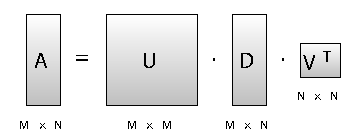
\includegraphics[width=0.75\textwidth]{img/svd_decomposition}
\end{figure}
\begin{itemize}
    \item $U$ is an $M\times M$ orthogonal matrix, $U^TU=I$
    \item $D$ is an $M\times N$ diagonal matrix
    \item $V^T$  is an $N\times N$ orthogonal matrix, $V^TV=I$ 
\end{itemize}
\subsection{Singular values}
The elements of $D$ are only non-zero on the diagonal and are called the \emph{singular values}. By convention, the order of the singular vectors is determined by the \emph{high-to-low} sorting of singular values, with the highest singular value in the upper left index of the $D$ matrix.
The first $r$ columns of $U$ are called \emph{left singular vectors}, they form an orthogonal basis for the space spanned by the columns of the original matrix $A$.

Similarly the first $r$ rows of $V^T$ are the \emph{right singular vectors}, they form an orthonormal basis for the row space of $A$.

SVD provides an explicit representation of the range and null-space of a matrix $A$.
\begin{itemize}
\item The right side singular vectors corresponding to vanishing singular values of $A$, span the null space of $A$:
\begin{align*}
d_i = 0 \quad \implies \quad Av_i = 0 \quad \implies \quad v_i \in Null(A).
\end{align*}
\item The left singular vectors corresponding to the non-zero singular values of $A$ span the range of $A$.
\end{itemize}
As a consequence, the rank of $A$ equals the number of non-zero singular values (= the number of non-zero elements in $D$).
\begin{align*}
Rank(A) = \# d_i > 0.
\end{align*}
\subsection{Closest Rank-$k$ Matrix}
Let the SVD of $A \in \R^{M\times N}$  be given by $A=UDV^T$. If $k<r = Rank(A)$ and
\begin{align*}
    A_k = \sum_{i=1}^k d_i u_i v_i^T.
\end{align*}
Then 
\begin{align*}
    \min_{Rank(B)=k} \norm{A-B}_2 = \norm{A-A_k}_2.
\end{align*}
This means that $A_k$ is the closest $Rank(k)$ approximation to $A$ in the Eculidean matrix norm sense hence:
\begin{align*}
    \norm{A-A_k}_2 = d_{k+1}.
\end{align*}

\subsection{Properties}
The columns of $U$ are the eigenvectors of $AA^T$. This claim can be verified using the SVD decomposition:
\begin{align*}
    AA^T = UDV^T VDU^T = UD^2U^T.
\end{align*}
Similarly the rows of $V^T$ (or columns of $V$) are the eigenvectors of $A^TA$ as:
\begin{align*}
    A^TA = VDU^T UDV^T = VD^2V^T.
\end{align*}



\newpage
\part{Clustering}

\section{Introduction}
A set of datapoints in a $d$-dimensional Euclidean space is given.
\begin{description}
    \item[Aim] The aim is to find a \emph{meaningful partition} of the data; i.e. label each data point with a unique value $\{1,\ldots, k\}$.
    \item[Objective] The partition should group together similar data points, while the different groups/clusters should be as dissimilar as possible from each other.
    \item This way we can uncover similarities between data points and give rise to data compression schemes.
\end{description}


\subsection{Problem}
Consider $N$ data points in a $D$-dimensional space. Each data vector is denoted by $x_n$, $n=1,\ldots,N$. Our goal is to partition the data set into $K$ clusters: Find vectors $u_1, \ldots, u_K$ that represent the centroid of each cluster.

A datapoint $x_n$ belongs to cluster $k$ if the Euclidean distance between $x_n$ and $u_k$ is smaller than the distance to any any other centroid.

Mathematically, the clustering problem defines a mixed discrete continuous optimisation problem. 

\subsubsection{The Cost Function of Vector Quantisation}
\begin{description}
    \item[Objective] Minimise the cost function
        \begin{align*}
            J(U,Z) = \norm{X-UZ}_F^2 = \sum_{n=1}^N\sum_{k=1}^K z_{k,n} \norm{x_n-u_k}_2^2
        \end{align*}
        where
        \begin{align*}
            X &= [x_1,\ldots, x_N] \in \R^{D\times N}\\
            U &= [u_1,\ldots, u_K] \in \R^{D\times K}, &\text{centroids}\\
            Z &\in \{0,1\}^{K\times N}, &\text{assignments}
        \end{align*}
        with $\sum_k z_{k,n} = 1 \forall n$ i.e.,  one element per columns set to $1$.
\end{description}
Assignment notation:
\begin{description}
    \item[Assignment Notation]: Vector $\hat z \in \{1,\ldots,K\}^N$ indicating for each data point to which cluster index it is assigned:
    \begin{align*}
        \hat z = \begin{pmatrix}
                    2\\ 3\\ 4\\ 2 \\ 2\\ 1
                 \end{pmatrix}
    \end{align*}
    \item[Matrix Notation]: The matrix $Z\in \{0,1\}^{K\times N}$ with only one non-zero entry per column, assigns data points to clusters:
    \begin{align*}
        Z &= \begin{pmatrix}
                 0&0&0&0&0&1\\
                 1&0&0&1&1&0\\
                 0&1&0&0&0&0\\
                 0&0&1&0&0&0
             \end{pmatrix}
    \end{align*}
\end{description}

\section{$K$-Means}
\subsection{Overview}

The algorithm alternates between two steps:
\begin{itemize}
    \item \emph{Assigning data points} to clusters
    Let $k^*(x_n)$ denote the cluster index with the minimal distance between a cluster centroid and the data point $x_n$:
    \begin{align*}
    k^*(x_n) &=\argmin_k \left\{ \norm{x_n-u_1}_2^2,\ldots, \norm{x_n-u_k}_2^2,\ldots,\norm{x_n-u_K}_2^2 \right\}
    \end{align*}

    \item \emph{Updating the cluster centroids} based on all the data points assigned to it. Compute the mean/centroid of a cluster that can be written as:
    \begin{align*}
        u_k = {\sum_{n=1}^N z_{k,n} x_n \over \sum_{n=1}^N z_{k,n} }\quad \forall k,\ \ k\in \{1,\ldots,K\}
    \end{align*}
\end{itemize}

\subsection{Algorithm}
\begin{enumerate}
\item Initiate with a random choice of $u_1^{(0)}, \ldots, u_K^{(0)}$ (or let $u_1^{(0)}, \ldots, u_K^{(0)}$ equal data points from the set). Set $t=1$.
\item \textbf{Cluster assignment.} Solve $\forall n$:
    \begin{align*}
        k^*(x_n) &=\argmin_k \left\{ \norm{x_n-u_1^{(t)}}_2^2,\ldots, \norm{x_n-u_K^{(t)}}_2^2 \right\}.
    \end{align*}
    Then, $z_{k*(x_n),n}^{(t)} = 1$ and $z_{j,n}^{(t)} =0\ \forall j\neq k,\ \ j=1,\ldots, K$.
\item \textbf{Centroid update} 
    \begin{align*}
        u_k^{(t)} = {\sum_{n=1}^N z_{k,n}^{(t)} x_n \over \sum_{i=1}^N z_{k,n}^{(t)}}\ \forall k,\ k\in\{1,\ldots,K\}
    \end{align*}
\item Increment $t$. Repeat step $2$ until $\norm{u_k^{(t)}-u_k^{(t-1)}}_2^2 < \varepsilon\ \forall K$ ($0<\varepsilon << 1$) or until $t=t_\text{finish}$.  
\end{enumerate}
Aspects:
\begin{itemize}
    \item The computational cost of each iteration is $\bigO{KN}$.
    \item Convergence is guaranteed
    \item Optimises a \emph{non-convex} objective. Hence only a local minimum can be guaranteed.
    \item Can be used to compress data: store only the centroids and the assignments of data point to clusters.
\end{itemize}
Problems:
\begin{itemize}
\item Non-convex objective, local minima and sensitive to initialisations.
\item Not appropriate for non-Euclidean data $\mapsto$ need to use other distances.
\item The optimal number of clusters $K$ is unknown: One has to find a balance between total compression $(K=1)$ and no loss of information $(K=N)$.
\end{itemize}

\subsection{Stability}
\subsubsection{High-Level Stability test}
The following is a high-level stability test for a given set of data points and a given number of clusters:
\begin{enumerate}
    \item Generate perturbed versions of the set for example by adding noise or drawing sub-samples.
    \item Apply the clustering algorithm on all versions.
    \item Compute pair-wise distances between all clusterings (using some distance measure).
    \item Compute the \emph{instability} as the mean distance between all clusterings.
\end{enumerate}
Repeat this for different numbers of clusters and choose the one that minimises the instability.
\subsubsection{Distance between Clusterings}
For two clusterings $C$ and $C'$ that are defined on the same data points we compute the distance between clusterings $d$ in the following procedure:
\begin{enumerate}
    \item Compute the distances between the two clusterings by counting points on which the two clusterings agree or disagree.
    \item Repeat over all permutations of the cluster labels (since the same cluster might be sometimes labeled $1$ and sometimes $2$ etc...).
    \item Choose the permutation with minimal distance and the corresponding distances is $d$.
\end{enumerate}
In other words,
\begin{align*}
    d = \min_\pi \norm{Z-\pi(Z')}_0
\end{align*}
where $\pi(Z')$ is one of the possible row permutations of $Z'$ and $\norm{Z}_0$ denotes the cardinality of $Z$.
If two clusterings are defined on different data sets but many points overlap, we use only these for comparison, otherwise, a mapping from one domain to the other is required.

\subsubsection{Calculation of Stability}
The rate of inconsistent data items $r$ is computed as follows"
\begin{enumerate}
    \item Cluster data sets $X$, $X'$ to infer assignments $Z$, $Z'$.
    \item Train a classifier $\phi$ on $(X,Z)$ to transfer the clustering results $Z$ on $X$ to $X'$.
    \item Apply $\phi$ on $X'$ and compare the optimally permuted output with $Z'$:
    \begin{align*}
        r:= {1\over N} \min_{\pi \in \mathbb S_K} \left\{ \sum_{i=1}^N \mathbb I_{\{ \pi(\phi(x_i'))\neq\hat z_i' \}}\right\}.
    \end{align*}
The indicator function $\mathbb I_{\{p\}}$ is $1$ if predicate $p$ is true, and $0$ otherwise.

Minimisation of $\pi\in \mathbb S_K$ compensates for the permutation of the cluster numbers.
\end{enumerate}
The higher the number of clusters, the more difficult it is to have a small rate $r$ of inconsistent cluster assignments. Given $K$ clusters of equal size, a random assignment yields
\begin{align*}
    r_{rand} = {K-1\over K}.
\end{align*}
To be able to compare hypotheses with different $K$, relate $r$ to $r_{rand}$. The \emph{stability} is this defined as:
\begin{align*}
    stab := 1 - {r \over r_{rand}}.
\end{align*}
\begin{itemize}
    \item $stab=1$: No inconsistent assignments
    \item $stab=0$: Not better than a random assignment
\end{itemize}

\section{Clustering as Matrix Factorisation}
SVD is a class matrix factorisation technique according to which every matrix matrix can be decomposed into $X=UDV^T$. With $U\in \R^{D\times D}$, $D\in \R^{D\times N}$ and $V\in \R^{N\times N}$.
By setting $UD$ in the decomposition as $U$ and renaming $V^T$ to $Z$, we can write
\begin{align*}
    X= UZ.
\end{align*}

Approximating $X$ using the $K$ largest singular values we get a factorisation involving matrices of the same dimensionality as $K$-Means. 




\section{Mixture Models}
\subsection{Soft Clustering}
The term Soft clustering is ambiguous since it can refer to the algorithm or to the model:
\begin{description}
\item[Algorithmic] Soft $K$-Means: Instead of assigning a point to exactly one cluster. Consider assigning a probability that a data point belongs to a certain cluster. 
\item[Model relaxation]
\end{description}

\section{Multi-Assignment Clustering}

\subsection{Role-Based Access Control (RBAC)}
Given a \emph{user-permission} matrix $X\in \mathbb B^{D\times N}$, find
\begin{description}
\item[Roles] $U\in \mathbb B^{D\times K}$ and
\item[Assignments] $Z\in \mathbb B^{K\times N}$ 
\end{description}
with $\mathbb B=\{0,1\}$ such that
\begin{align*}
    X = U \otimes Z \quad \Leftrightarrow \quad x_{dn} = \bigvee_k [u_{dk} \land z_{kn}].
\end{align*}
\begin{itemize}
\item Each role defines a set of permissions
\item Users are assigned to a set of roles and get all permissions of these roles.
\end{itemize}

\subsubsection{Notation}
\begin{itemize}
\item $x_{dn} \in \{0,1\}$: Assignment of user $n$ to permission $d$.
\item $z_{kn} \in \{0,1\}$: Assignment of user $n$ to role $k$.
\item $u_{dk} \in \{0,1\}$: Assignment of permission $d$ to role $k$.
\item $\beta_{dk} \in [0,1]$: Probability of $u_{dk} = 0$.
\end{itemize}
\begin{figure}[H]
    \centering
    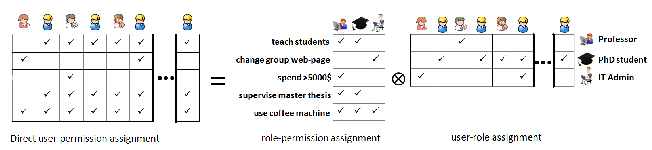
\includegraphics[width=\textwidth]{img/multi_assignment_rbac}
\end{figure}

\subsubsection{Evaluation Criteria}
For each role mining problem definition, there is a (set of) evaluation criteria:
\begin{itemize}
\item Matrix Reconstruction
\item Number of Sources
\item Inference Quality
\item Generalisation
\item Stability
\end{itemize}

\subsection{Binary Matrix Factorisation}
\emph{Min-Noise Approximation}: Given $K$, find the matrices $\hat U$, $\hat Z$ such that
\begin{align*}
    (\hat U, \hat Z) =\argmin_{U,Z} \norm{X-U\otimes Z}_1
\end{align*}
with $U\in \mathbb B^{D\times K}$ and $Z\in \mathbb B^{K\times N}$. This problem is also called \emph{approximate Boolean Matrix decomposition} and has the following properties:
\begin{itemize}
    \item \textbf{All} matrices are Boolean,
    \item It is a \emph{combinatorial optimisation problem},
    \item It is proven to be \emph{NP-hard} (reducible to set basis problem).
\end{itemize}
In contrast to recommender systems a the outputs $\hat U$ and $\hat Z$ are always binary.

\subsubsection{Rounded SVD}
\begin{enumerate}
    \item Compute the singular value decomposition
        \begin{align*}
            X=U\cdot S\cdot V^T
        \end{align*}
    \item Discard columns $K+1,\ldots,D$ of $U$ to get $U_{(K)}$.\\
          Discard rows $K+1,\ldots,N$ of $V$ to get $V_{(K)}$.
    \item Round the left and right singular vectors to get Boolean matrices $\hat U$ (roles) and $\hat Z$ (role assignments):
        \begin{align*}
            \hat U &= (U_{(K)} > t_U)\\
            \hat Z &= (V_{(K)} > t_V)
        \end{align*}
        where $t_U$ and $t_V$ are thresholds.
\end{enumerate}
The rounded continuous decomposition is a poor Boolean decomposition!

\subsubsection{$K$-means}
$K$-means partitions objects into disjoint groups (clusters) s.t. the average \emph{distance} between data and corresponding cluster prototypes is minimal. 
The standard objective function for $K$-means uses the \emph{Euclidean distance} measure:
\begin{align*}
    J(U,Z) = \norm{X-UZ}_2^2 = \sum_{n=1}^N \sum_{k=1}^K z_{kn} \norm{x_n - u_k}_2^2
\end{align*}
and centroids are updated via mean operation.

In order to use $K$-means for a Boolean decomposition the distance is adapted to use \emph{Hamming distance} (0-norm):
\begin{align*}
    J(U,Z) = \norm{X-UZ}_0 = \sum_{n=1}^N \sum_{k=1}^K z_{kn} \norm{x_n - u_k}_0
\end{align*}
The centroids $u_k$ are restricted to Boolean values and the centroid update step needs to be adapted:
\begin{align*}
    u_{dk} = \text{median}(\{x_{dn}|z_{kn} =1 \})\ \forall k\in \{1,\ldots,K\},\ \forall d \in \{1,\ldots, D\}
\end{align*}

$K$ can be found with cross-validation. $K$-means only yields \emph{disjoint clustering}, i.e. $Z$ matrix has only a single $1$ in each column. In RBAC however a user can have multiple role. 

\subsubsection{RoleMiner}
RoleMiner is a heuristic for role mining. Idea: A set of common permissions could potentially be a role. Roles are created by finding common sets of permissions between user.

Comes in two variants: \emph{CompleteMiner} and \emph{FastMiner}.

RoleMiner is very sensitive to noise:
\begin{itemize}
    \item If only a few individual bits are noisy, then the number of candidate roles gets much larger.
    \item The result is unstable: If the noise changes slightly, then the solution is completely different.
\end{itemize}

\subsubsection{DBPsolver}
DBPsolver approximately solves the \emph{Discrete Basis Problem}.
\paragraph{Discrete Basis Problem:} For a given Boolean matrix $X\in \mathcal B^{D\times N}$ and a number $K$ of basis vectors, find a Boolean matrix $U\in \mathcal B^{D\times K}$ and a Boolean matrix $Z\in \mathcal B^{K\times N}$ minimising 
\begin{align*}
    \norm{X-U\otimes Z}_F^2.
\end{align*}
The discrete basis problem and min-noise Role Mining problem are identical.

\subsubsection{Probabilistic Clustering}
\paragraph{Difficulties so far}
\begin{itemize}
 \item Searching in the full Boolean spaces has a \emph{too high complexity}.
 \item Restricting the Boolean search spaces \emph{ignores solutions}
 \item Searching solutions in continuous space and rounding \emph{produces poor results}.
 \item Search heuristics are prone to \emph{overfitting}
\end{itemize}

\paragraph{Modeling of RBAC} Computing a likelihood requires to design a probabilistic model $p(X|U,Z)$ for the generation process of the data $X$. This is the probability $X$ given the model, the cluster assignments $Z$, and the cluster centroids $U$.

\paragraph{Derivation I: One Object} For the simple case we consider one cluster per object:
\begin{align*}
\sum_k z_{kn} = 1, \qquad \forall n \in \{1, \ldots, N\}.
\end{align*}
$k_n$ is the cluster of object $n$: 
\begin{align*}
    k_{n} = \{ k\in \{1, \ldots, L\}| z_{kn} = 1\}.
\end{align*}
Consider on entry $x_{dn}$:\todo{WTF}
\begin{align*}
    p(x_{dn} = 0 | \beta_{d\cdot},z_{\cdot n}) = \beta_{dk_n}.
\end{align*}
Therefore:
\begin{align*}
    p(x_{dn} = 1 | \beta_{d\cdot},z_{\cdot n}) &=  1 - p(x_{dn} = 0 | \beta_{d\cdot},z_{\cdot n})\\
        &= 1-\beta_{dk_n}
\end{align*}

\paragraph{Derivation II: All objects} Objects are now independent given the parameters $Z$ and $U$. Thus:
\begin{align*}
    p(X|\beta,Z) &= \prod_{n=1}^N \prod_{d=1}^D p(x_{dn} = 1 | \beta_{d\cdot},z_{\cdot n})^{x_{dn}}\cdot p(x_{dn} = 0 | \beta_{d\cdot},z_{\cdot n})^{1-x_{dn}}\\
     &= \prod_{n,d} (1-\beta_{dk_n})^{x_{dn}} \beta_{dk_n}^{1-x_{dn}}
\end{align*}

\subsubsection{Multi-Assignment Clustering}
Compared to probabilistic clustering we don't restrict an object to one cluster.

One $x_{\cdot n}$ is generated by a \emph{set of clusters} $\mathcal L_n := \{k|z_{kn} = 1\}$. The resulting Boolean features are generated by \emph{disjunction} of the corresponding Boolean cluster centroids $u_{k,}$ (logical OR).
\begin{figure}[H]
    \centering
    
\includegraphics[width=0.8\textwidth]{img/multi_assignment_clustering}
    \caption{An object as the disjunction of the three clusters it belongs to.}
\end{figure}

\paragraph{Probabilistic view:} An object being generated by two clusters $k_1$, $k_2$ has probability $\beta_{dk_1}\beta_{dk_2}$ to have a $0$ at this dimension. 

Generally, an object $n$ belonging to the set of clusters $\mathcal L_n := \{ k|z_{kn} = 1\}$ has a probability $\beta_{\mathcal L_n} := \prod_{k\in \mathcal L_n} \beta_{dk}$ for a $0$ at dimension $d$.


In turn, it holds that $p(x_{dn}=1|z,\beta) = 1-\beta_{\mathcal L_n}$. Thus we get the following model:
\begin{align*}
    p(X|\beta, Z) = \prod_{n,d} \underbrace{\left(1-\prod_k \beta_{dk}^{z_{kn}} \right)^{x_{dn}} }_{\text{Noise component}} \underbrace{\left(\prod_k \beta_{dk}^{z_{kn}}\right)^{1-x_{dn}}}_{\text{Signal component}}
\end{align*}
\todo{Not sure about the component naming}

\subsubsection{Noise model for RBAC}

The deterministic RBAC generation of $X$:
\begin{align*}
    X = U\otimes Z \quad \Leftrightarrow\quad  x_{dn} = \bigvee_k [u_{dk} \land z_{kn}].
\end{align*}
Since this generation rule is not able to explain erroneous assignments in $X$ as noise we introduce a \emph{mixture noise model}:
\begin{align*}
    x_{dn} = (1-\xi_{dn})(U\otimes Z)_{dn} + \xi_{dn}\eta_{dn}
\end{align*}
where $\xi_{dn}$ is a binary noise indicator and $\eta_{dn}$ is a binary random variable.

\paragraph{Mixture Noise Model} Noise generation:
\begin{itemize}
    \item $\xi_{dn}$ indicates whether a bit is generated by $p_N (\xi_{dn}=1)$ or by $(U\otimes Z)_{dn}(\xi_{dn}=1)$. $\xi_{dn}$ is Bernoulli distributed:
    \begin{align*}
        p(\xi_{dn}|\varepsilon) = \varepsilon^{\xi_{dn}} (1-\varepsilon)^{1-\xi_{dn}},
    \end{align*}
    where $\varepsilon$ is the probability to choose a random bit.
    \item If the bits is noisy ($\xi_{dn}=1$), draw $\eta_{dn} = x_{dn}$ from
    \begin{align*}
        p_N(x_{dn}|r) = r^{x_{dn}} (1-r)^{1-x_{dn}},
    \end{align*}
    with $r$ being the probability that a noisy bit is $1$ ie. a user exceptionally gets a permission.
\end{itemize}
This can be modelled to a structure model:
\begin{align*}
    p_S(X|\beta, Z) = \prod_{n,d} \left( 1-\prod_k (\beta_{dk})^{z_{kn}}\right)^{x_{dn}} \left( \prod_k (\beta_{dk})^{z_{kn}}\right)^{1-x_{dn}},
\end{align*}
with $\beta_{dk}=p(u_{dk}=0)$.

This then can be combined with the noise model:
\begin{align*}
    p(X|Z, \beta, \xi, r) &= \prod_{n,d} p_N(x_{dn}|r)^{\xi_{dn}} p_S(x_{dn}|\beta_{d\cdot}, z_{\cdot n})^{1-\xi_{dn}}\\ 
    &= \prod_{n,d} \underbrace{\left( r^{x_{dn}}(1-r)^{1-x_{dn}}\right)^{\xi_{dn}}}_{x_{dn}\text{ generated by noise}}
    \underbrace{
        \left(\left[1-\prod_k (\beta_{dk})^{z_{kn}}\right]^{x_{dn}} 
            \left[ \prod_k(\beta_{dk})^{z_{kn}} \right]^{1-x_{dn}}
        \right)^{1-\xi_{dn}}
    }_{x_{dn}\text{ generated by roles}}.
\end{align*}

The $\xi_{dn}$ are unobservable (hidden) variables:
\begin{itemize}
\item They are unknown.
\item They are too many to be estimated.
\end{itemize}

We thus integrate the $\xi$ out of $p(X|Z,\beta, \varepsilon, \xi, r)$:
\begin{align*}
    p(X|Z,\beta,\varepsilon,r) = \sum_{\{\xi\}} p(X,\xi|Z,\beta, \varepsilon,r),
\end{align*}
where
\begin{align*}
    p(X,\xi|Z,\beta, \varepsilon, r) &=
        p(X|Z,\beta,\xi, r)p(\xi|\varepsilon)\\
        &= p(X|Z,\beta,\xi, r)\prod_{n,d}\varepsilon^{\xi_{dn}} (1-\varepsilon)^{1-\xi_{dn}}\\
        &= \prod_{n,d} \left(\varepsilon r^{x_{dn}} (1-r)^{1-x_{dn}}\right)^{\xi_{dn}}
            \left((1-\varepsilon)(1-\beta_{d,\mathcal L_n})^{x_{dn}}(\beta_{d,\mathcal L_n})^{1-x_{dn}}\right)^{1-\xi_{dn}}.
\end{align*}

\paragraph{Mixture Model:}
The likelihood function can thus be written as:
\begin{align*}
    p(X|Z,\beta,\varepsilon,r) &=
        \prod_{n,d} \left( \varepsilon r^{x_{dn}} (1-r)^{1-x_{dn}}+(1-\varepsilon)(1-\beta_{d,\mathcal L_n})^{x_{dn}} (\beta_{d,\mathcal L_n})^{1-x_{dn}} \right)\\
        &=  \prod_{n,d} \left(\varepsilon r + (1-\varepsilon)(1-\beta_{d,\mathcal L_n})\right)^{x_{dn}}
        \left(\varepsilon (1-r)+(1-\varepsilon)\beta_{d,\mathcal L_n}\right)^{1-x_{dn}}
\end{align*}
Parameters to estimate:
\begin{itemize}
    \item $Z$: user-role assignments.
    \item $\beta$: probabilities of role-permission assignments $U$ to be $0$.
    \item $\varepsilon$: noise probability.
    \item $r$: probability of noisy bits to be $1$.
\end{itemize}

This function requires a non-convex objective function to maximise the log-likelihood.

\section{Non-Negative Matrix Factorisation}

Problem:
\begin{itemize}
    \item Given: Corpus of text documents such as web pages
    \item Goal: Find a low-dimensional representation of these documents. 
\end{itemize}

\paragraph{Document Representation}
\begin{description}
\item[Vocabulary] Every semantically "useful"word in a language. This excludes all the stop words (the, is, at, which, etc...). Stemming reduces the text to it's root form: Cats, catlike, catty, etc. all map to the same word "cat".


$D$ denotes the size of the vocabulary.

\item[Document] \emph{Bag of words}-model: Ordering of the words in a document is ignored. The document is represented by a vector of length $D$ with frequencies/counts of different words. This vector is usually very sparse.
\end{description}

\subsection{Matrix view} Here $N$ denotes the number of documents and $K$ denotes the number of "clusters" with $D$ being the vocabulary size.
\begin{itemize}
    \item $X \in \R_+^{D\times N}$ denotes the document-term matrix which stores the word counts for each document:
        \begin{align*}
            X = [x_1,\ldots, x_N]
        \end{align*}
        $x_{dn}$: Frequency of the $d$-th word in the $n$-th document.
    \item We study a non-negative matrix factorisation (NMF) of the document matrix $X$:
        \begin{align*}
            X\approx UZ
        \end{align*}
        with $U\in \R_+^{D\times K}$ and $Z\in \R_+^{K\times N}$, with $\R_+ := [0,\ldots, \infty)$ . 
\end{itemize}
\subsection{Methods}
\subsubsection{Full Singular Value Decomposition}
A singular value decomposition can be used to decompose the document word matrix:
\begin{align*}
    X = U\Sigma V^T.
\end{align*}
However the procured $U$ and $V$ are not guaranteed to be non-negative. 

\subsubsection{Classic Latent Semantic Indexing (LSI)}
The LSI method uses a partial SVD
\begin{align*}
    \tilde X = U\tilde \Sigma V^T \approx X.
\end{align*}
With $\tilde \Sigma$ having all but the largest $K$ singular values set to zero. 

\paragraph{Mapping function} A query $x$ can now be mapped by the query can now be compared/queried with an inner product:
\begin{align*}

\end{align*}


\newpage
\part{Sparse Coding}
A signal and its representation are not the same thing. There are an infinite number of possible representation, each capturing different  characteristics of the signal. 

Natural signals have a \emph{sparse representation} in a suitable dictionary due to regularity. Sparsity means that many coefficients vanish, e.g. have zero (or close to zero)  magnitude.
\section{Signal Compression}
Given original signal $x$ and given an orthogonal matrix $A$. Compute the linear transformation (change of basis) $z=Ax$. Truncate "small" values of $z$ which yields an estimate $\hat z$. Compute the inverse transform $\hat x = A^T \hat z$.


The key idea being the \emph{orthogonality} of $A$.

\paragraph{Compressions Algorithm} $\ $
\begin{description}
\item Given an original signal $x$ and an \emph{orthogonal matrix $A$}.
\item Compute the linear transformation (change of basis) $z=Ax$. 
    \subitem Since $A$ is orthogonal, the transformed vector $z$ has the same "energy" as the original signal $x$.
\item Truncate "small" values, giving $\hat z$.
    \subitem We are interested in a \emph{sparse signal}, that is we want $z$ with a small number $K$ of non-zeros.
    \subitem We have compressed the signal since we only need to store $K$ values.
    \subitem The compression is lossy since we have discarded elements of $z$ (by setting them to zero).
\item Compute the inverse transform $\hat x = A^T \hat z$.
    \subitem Since $A^{-1} = A^T$ computing the inverse transform is efficient.
\end{description}

\paragraph{Decomposition and Reconstruction} $\ $
\begin{description}
\item Given a signal $f$ and an orthonormal basis $\{u_1,\ldots, u_L\}$.
\item The coefficients representing signal $f$ in the basis are given by 
    \begin{align*}
        z_l = \langle f, u_l \rangle,
    \end{align*}
    that is $f$ can be reconstructed by
    \begin{align*}
         f=\sum_{l=1}^L z_lu_l = \sum_{l=1}^L \langle f,u_l\rangle u_l.
    \end{align*}
\item Setting certain coefficients $z_l$ to zero is equivalent to not using certain basis functions $u_l$ that is for a subset $\sigma$  of size $K$,
    \begin{align*}
        \hat f = \sum_{k\in \sigma} z_ku_k.
    \end{align*}
\item The reconstruction error is given by
    \begin{align*}
        \norm{f-\hat f}^2 = \sum_{k\notin \sigma} |\langle f,u_k\rangle|^2,
    \end{align*}
    since $\langle u_k, u_l\rangle = 0$ for $k\neq l$.
\end{description}

\subsection{Fourier Basis}
\begin{align*}
 \hat f(\xi) &= \int_{-\infty}^\infty f(x) e^{-2\pi ix\xi} dx & \forall x \in \R\\
 f(x) &= \int_{-\infty}^\infty \hat f(x) e^{2\pi i\xi x}d\xi & \forall x\in \R
\end{align*}

\subsection{Haar Wavelets}
\begin{figure}[H]
\centering
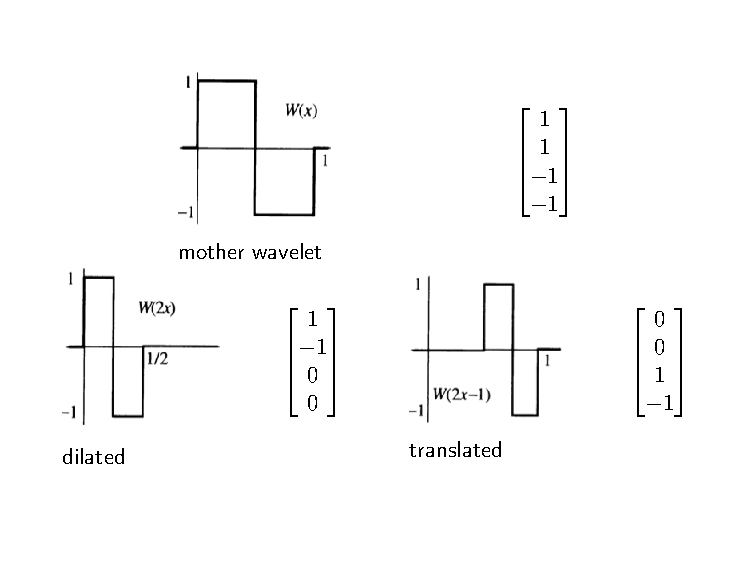
\includegraphics[width=0.7\textwidth]{img/08_haar_wavelets}
\end{figure}


\subsection{Fourier Basis vs Wavelet Basis}
\begin{description}
\item[Fourier Basis] $\ $
    \begin{itemize}
    \item Global support
    \item Good for "sine like" signals
    \item Poor for localised signals
    \end{itemize}
\item[Wavelet Basis] $\ $
    \begin{itemize}
    \item Local support
    \item Good for localised signals
    \item Poor for non-vanishing signals.
    \end{itemize}
\end{description}


\section{Principal Component Analysis (PCA)}
Given $X=[x_1,\ldots, x_N]$ a set of vectors we want to compress. Compute the (centered) covariance matrix:
\begin{align*}
    \Sigma = {1\over N} (X-M)(X-M)^T.
\end{align*}
Compute the eigenvector decomposition:
\begin{align*}
    [U\Lambda] = eig(\Sigma).
\end{align*}
Note that since $\Sigma$ is symmetric $U$ is an orthonormal matrix. Choose $K$ eigenvectors corresponding to the largest eigenvalues $U_K$.

For a given signal $x$ the compressed coefficients are
\begin{align*}
    \hat z = U_K x.
\end{align*}
Also known as the Karhunen-Loeve transform or Hoteling transform.

\subsubsection{Communication Cost}
\begin{description}
\item[PCA Basis] $\ $
    \subitem The basis $U_k$ is dependent on the data and is optimal for the given covariance.
    \subitem Need to transmit both the basis $U$ and the elements of $\hat z$.
\item[Fixed Basis] $\ $
    \subitem Both parties (compressor and decompressor) agree upon a particular basis, e.g. Haar Wavelets.
    \subitem Hence we only need to transmit the non-zero elements of the transformed signal $\hat z$.
\end{description}

\subsection{Compressive Sensing}
Assume that the original signal $x\in \R^D$ is sparse in some orthonormal basis $U$ with $K$ large coefficients in its sparse representation $z$:
\begin{align*}
    x= Uz,\qquad \text{s.t. }|I_{z>>0}| = K.
\end{align*}

The main idea of this method is to acquire the set $y$ of $M$ linear combinations of the initial signal instead of the signal itself and then reconstruct the initial signal from the measured one. 
\begin{align*}
    y_k &= \langle w_k, x\rangle,\ k=1,\ldots,M\\
    y &= Wx = WUz =: \Theta z &\text{with } \Theta = WU \in \R^{M\times D}.
\end{align*}


Surprisingly given any orthonormal basis $U$ we can obtain a stable reconstruction for any $K$-sparse and compressible signal.

This is true under two conditions:
\begin{align*}
    \item All elements $w_{i,j}$ of matrix $W$ are i.i.d. random variables with a Gaussian distribution with zero mean and variance ${1\over D}$.
    \item $M:M \geq cK\log\left({D\over K}\right)$, where $c$ is some constant.
\end{align*}

To recover the initial signal $x\in \R^D$ from the measured signal $y\in \R^M$ we need to find a sparse representation $z$:
\begin{align*}
    y = Wx = WUz = \Theta z, \qquad \Theta \in \R^{M\times D}.
\end{align*}

Given $z$ we can easily construct $x$:
\begin{align*}
    x = Uz.
\end{align*}

The problem of finding $z$ appears to be \emph{ill-posed} as $M<<D$: Since there are many more unknowns than equations.

Generally this problem is NP hard. Using an approximation scheme like Matching Pursuit is recommended.

\subsection{Sparse Coding}
\begin{description}
\item[Coding via orthogonal transforms] Given original signal $x$ and orthogonal matrix $A$
    \begin{itemize}
        \item Compute linear transformation
            \begin{align*}
                z = Ax
            \end{align*}
        \item Truncate "small" values, giving $\hat z$.
        \item Compute inverse transform (recall $A^{-1} = A^T$)
            \begin{align*}
                \hat x = A^T \hat z
            \end{align*}
    \end{itemize}
\item[Measuring Performance] Sparsity and low reconstruction error.
    \begin{itemize}
        \item Measure the reconstruction error 
            \begin{align*}
                \norm{x-\hat x}.
            \end{align*}
        \item Measure the sparsity of the coding vector $z$ that is $nnz(z)$.
    \end{itemize}
\item[Dictionary Choice] General considereations
    \begin{itemize}
        \item Fourier dictionary is good for "sine like" signals.
        \item Wavelet dictionary is good for localised signals.
    \end{itemize}
\item[Compressive Sensing] $\ $
    \begin{itemize}
        \item Gather and store already compressed signal.
        \item Use $l_0$-norm minimisation to recover initial signal.
    \end{itemize}

\end{description}




























\section{Overcomplete Dictionaries}
\subsection{Introduction}
\emph{Overcompleteness} $(L>D)$: More atoms (dictionary elements) than dimensions.

\subsection{Morphology of Signals}
Different dictionaries are appropriate for different kinds of signals.

\paragraph{Dictionary selection Strategy} Either choose the appropriate dictionary manually or try several and choose the one which affords sparsest coding.

\subsubsection{Unions of Bases} 
\emph{Union of orthonormal bases} $[U_1\ldots U_B] \in \R^{D\times (B\cdot D)}$
\begin{figure}[H]
    \centering
    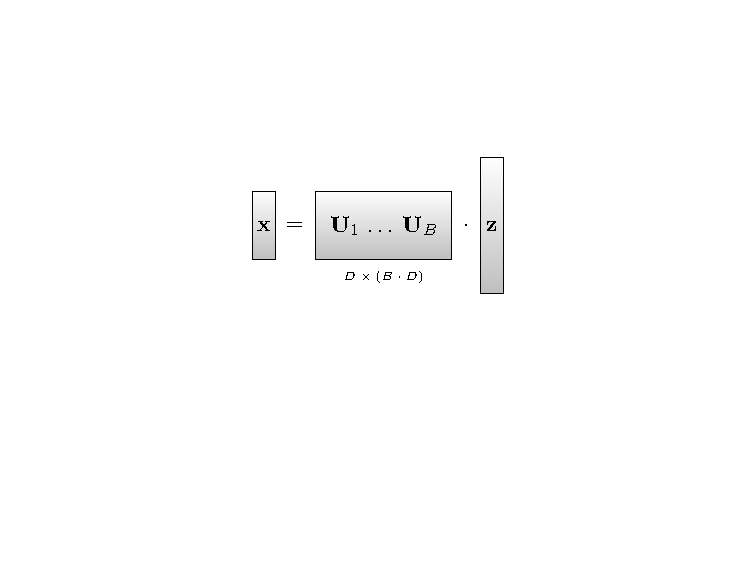
\includegraphics[width=0.6\textwidth]{img/09_union_of_bases}
\end{figure}
Each basis $U_b$ is responsible for one characteristic of the signal, and the total number of atoms is $K=B\cdot D$.

\subsection{General Overcomplete Dictionaries}
Consider the data set $\{x_1,\ldots, x_{10000}\}\in \R^3$:
\begin{figure}[H]
    \centering
    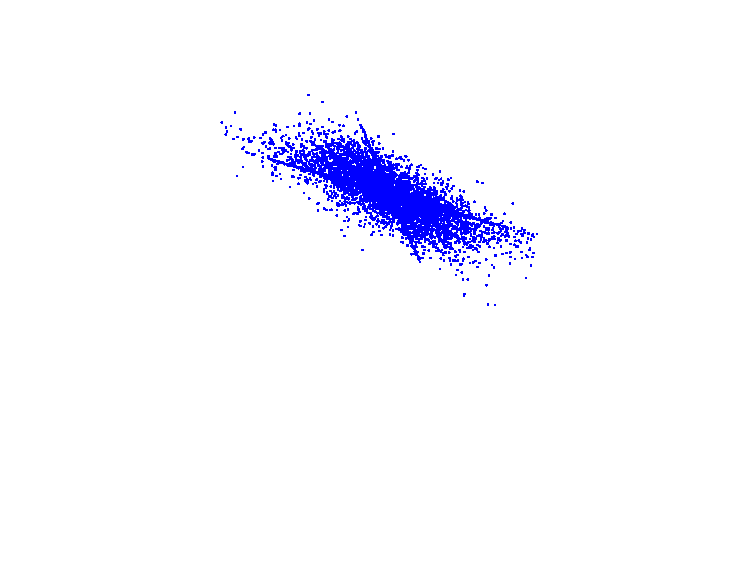
\includegraphics[width=0.6\textwidth]{img/09_overcomplete}
\end{figure}
\begin{itemize}
\item Full coding $(K=3)$ in spanning basis $U\in \R^{3\times 3}$.
\item $K=2$ coding possible using a four atom dictionary:
    \begin{align*}
         \tilde U = [u_1 u_2 u_3 u_4]\in \R^{3\times 4}
    \end{align*}
    aligned with densely populated subspaces.
\item $L>D$ atoms are no longer linearly dependent.
\end{itemize}

\paragraph{Example: Directional Gabor Wavelets} Directional oscillation, amplitude modulated by Gaussian window:
\begin{align*}
    g(n_1, n_2; \mu_1, \mu_2,f\theta) \propto 
        \exp\left[ 
             -(n_1-\mu_1)^2
            \right]
        \exp\left[
                -(n_2-\mu_2)^2
            \right]
        \times \Re \left\{
                        \exp \left[
                                i\cdot f\cdot (n_1\cos\theta+n_2\sin\theta)
                            \right]
                    \right\}
\end{align*}
\begin{figure}[H]
    \centering
    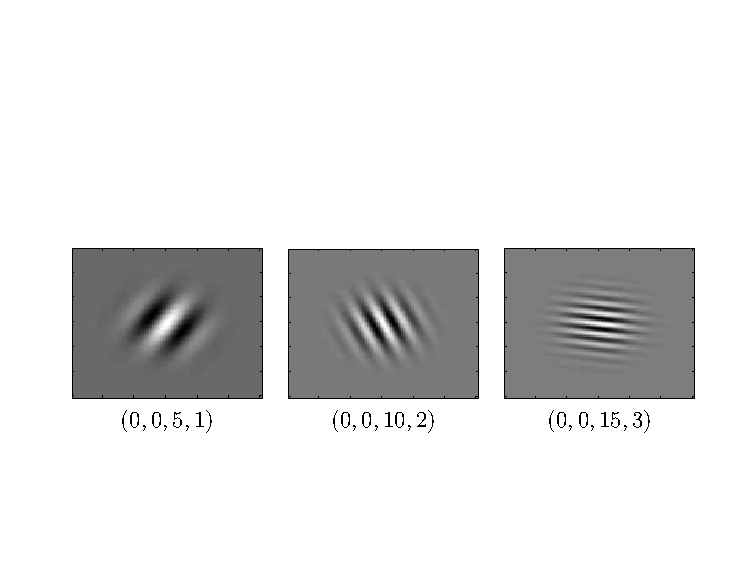
\includegraphics[width=0.8\textwidth]{img/09_gabor}
\end{figure}

\subsection{Coherence}
Increasing the \emph{over-completeness factor} ${L\over D}$:
\begin{itemize}
    \item Potentially increases the sparsity of the coding
    \item Increases the linear dependency betwee atoms.
\end{itemize}

Linear dependency measure for dictionaries: \emph{coherence}
\begin{align*}
    m(U) = \max_{i,j:\ i\neq j} \left| u_i^T u_j \right|
\end{align*}
\begin{description}
    \item $m(B)=0$ for an orthogonal basis $B$.
    \item $m([Bu]) \geq {1\over \sqrt{D}} $ if atom $u$ is added to $B$.
\end{description}

\subsection{Signal Coding}
\begin{description}
\item $U$ is \emph{orthonormal}:

    Matrix multiplication $z=U^T x$
\item $U$ is a \emph{spanning basis} ($D$ linearly dependent atoms):

    \begin{itemize}
        \item $z = U^{-1}$
        \item inverting $U$ can be ill-conditioned.
    \end{itemize}
\item $U \in \R^{D\times L}$ is \emph{overcomplete}:
    \begin{itemize}
        \item \emph{Ill-posed} problem: more unknowns than equations
        \item Have to add constraint: Find sparsest $z$ such that the equation holds:
            \begin{align*}
                 &z^* = \argmin_{z} \norm{z}_0\\
                 \text{s.t.}& x= Uz,
            \end{align*}
            where $\norm{z}_0$ counts the number of non-zero elements in $z$.
            
            \subitem $\norm{\cdot}_0$ is piece-wise constant.
            \subitem Finding the sparsest solution $z^*$ is NP hard (combinatorial problem).
            \subitem Brute-force approach: Try all possible atom subsets with $|\Delta| \leq D$.
            \subitem Needs an approximation scheme for realistic problem instances.
    \end{itemize}
\end{description}

\subsection{Noise Observations}
\subsubsection{Additive Noise}
\begin{align*}
     x = Uz + n
\end{align*}
Assumes each dimension is independently corrupted by zero-mean Gaussian nois:
    \begin{align*}
        n_d  \sim \mathcal N(0,\sigma^2)
    \end{align*}
    with variance $\sigma^2$.
    
\paragraph{Solve} by maximising the sparsity of $z$, while the \emph{residual} (approximation error) remains below $\sigma$:
\begin{align*}
     &z^*  = \argmin_{z} \norm{z}_0\\
     \text{s.t.}&\qquad \norm{x-Uz}_2 < \sigma
\end{align*}
or alternatively:

Minimise the residual while selecting less than $K$ atoms from the dictionary:
\begin{align*}
    &z^* = \argmin_z \norm{x-Uz}_2\\
    \text{s.t.}&\norm{z}_0 \leq K
\end{align*}

\subsubsection{Approximate Sparse Coding}
Explain the signal accurately with few atoms:
\begin{align*}
    x =Uz + n = Uz+Uy = U(z+y),    
\end{align*}
where $y$ is the coding of $n$ in $U$:
\begin{figure}[H]
    \centering
    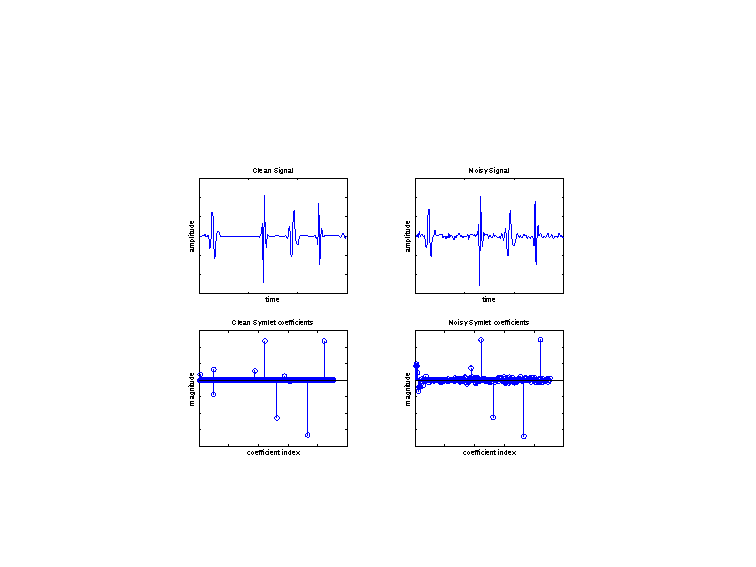
\includegraphics[width=0.7\textwidth]{img/09_noise_vs_signal}
\end{figure}
We observe that \emph{noise cannot be sparsely coded} in any dictionary, therefore $y$ has many small coefficients. Large coefficients are still due to $z$.

\paragraph{Geometry} of the sparse coding solution $z^*$:
\begin{figure}[H]
\centering
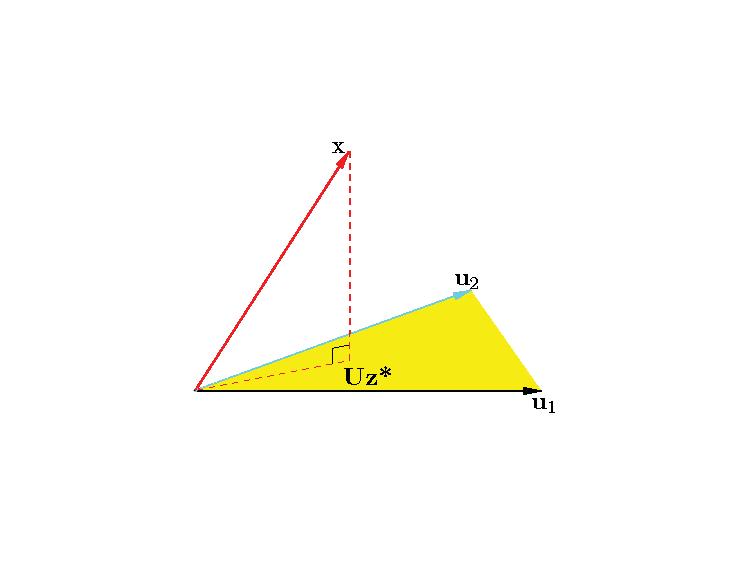
\includegraphics[width=0.5\textwidth]{img/09_geometry}
\end{figure}

The orthogonal projection of $x$ onto the subspace spanned by the selected atoms $\{u_d| z_d^* \neq 0\}$ minimises $\norm{x-Uz}_2$.

\section{Matching Pursuit}
Matching pursuit is a \emph{Greedy} algorithm: Thus approximates a NP hard problem iteratively each time taking the action which is short-term optimal.

\paragraph{Application to sparse coding:}$\ $
\begin{enumerate}
    \item Start with the zero vector $z=0$ and residual $r^0 = x$.
    \item At each iteration $t$, take a step in the direction of the atom $u_{d^*(t)}$ that maximally reduces the residual $\norm{x-Uz}_2$.
\end{enumerate}

\subsection{Minimising the Residual}
Atom selection at iteration $t$:
\begin{align*}
    d^{*} (t) = \argmax_d |\langle r^t, u_d\rangle|
\end{align*}

\paragraph{Proof} for the first iteration:
\begin{enumerate}
    \item Project $r^0 - x$ on atom $u_d$, to get
        \begin{align*}
            x = \langle x,u_d\rangle u_d + r^1
        \end{align*}
    \item Since $r^1$ is orthogonal to $u_d$, and $u_d^T u_d = 1$,
        \begin{align*}
            \norm{x}_2^2 = |\langle x,u_d\rangle|^2 + \norm{r^1}_2^2.
        \end{align*}
    \item Therefore, $\norm{r^1}_2^2$ is minimised by maximising $|\langle r^0, u_d\rangle|^2$.
\end{enumerate}



\subsection{Matching Pursuit Algorithm}
\begin{description}
\item[Objective] $\ $
    \begin{align*}
        z^* &= \argmin_z \norm{x-Uz}_2,\\
        \text{s.t }\ \norm{z}_0 &\leq K.
    \end{align*}

\item[Algorithm] $\ $
    \begin{algorithmic}
        \STATE $z\gets 0$
        \STATE $r\gets x$
        \WHILE{$\norm{z}_0 < K$}
            \STATE Select atom with maximum absolute correlation to residual:
                \begin{align*}
                 d^* \gets \argmax_d \left|  u_d^T r \right|
                \end{align*}
            \STATE Update coefficient vector and residual:
                \begin{align*}
                     z_{d^*} &\gets z_{d^*} + u_{d^*}^Tr\\
                     r &\gets r-\left( u_{d^*}^R r\right) u_{d^*}.
                \end{align*}
        \ENDWHILE
    \end{algorithmic}
\end{description}


\subsection{Discussion}
Assume $x=Uz$ has a $K$ sparse coding
\begin{align*}
 x=\sum_{d\in \Delta} z_d u_d.
\end{align*}

Under which condition is MP successful in recovering the true \emph{support}
\begin{align*}
    \Delta_{MP} = \Delta,
\end{align*}
where $\Delta_{MP} = \{d|z_{d^*} \neq 0\}$ is the set of coding atoms for the MP solution $z^*$?
Ie. when is the greedy approximation exact?

\begin{enumerate}
    \item Generate dictionary with atoms uniformly sampled on hypersphere.
    \item Generate observations with $K$ sparse coding.
\end{enumerate}
Compare $\Delta_{MO}$ with $\Delta$:

\begin{figure}[H]
    \centering
    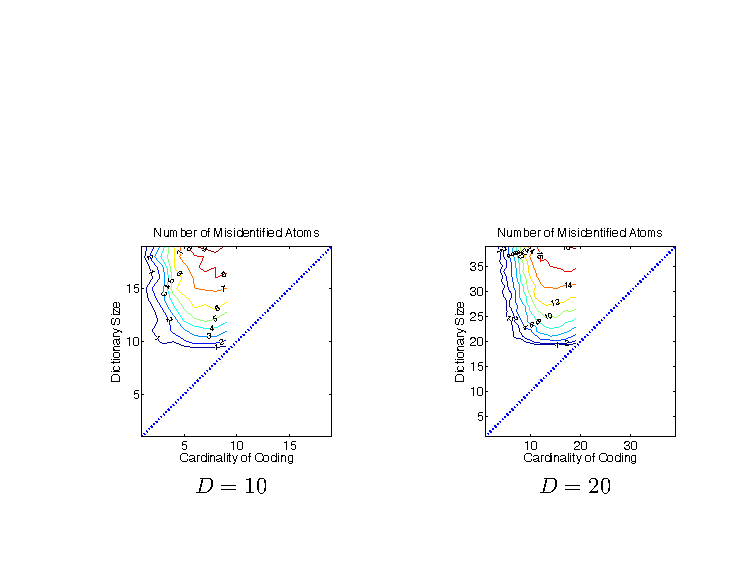
\includegraphics[width=0.7\textwidth]{img/09_mp_recovery}
\end{figure}
We observe that the recovery is possible even for $L>D$ if the true coding is \emph{sparse enough}.

\paragraph{Exact recovery condition}
    \begin{align*}
     K < {1\over 2} \left( 1+{1\over m(U)}\right)
    \end{align*}
guarantees support recovery by matching pursuit.


\begin{description}
\item Intuition: If the coherence is small, explaining a generating atom with other atoms is not sparse. Therefore sparse coding recovers support.
\item Trade-Off: Increasing L
    \begin{itemize}
        \item Leads to sparser coding (smaller possible $K$),
        \item But it increases coherence $m(U)$.
    \end{itemize}
\end{description}

\subsection{Inpainting}
\paragraph{Idea} $\ $
\begin{enumerate}
\item Sparse coding of known parts of the image,
\item Predicting missing parts by reconstruction from sparse code.
\end{enumerate}
\paragraph{Algorithm} $\ $
\begin{enumerate}
    \item Define a diagonal masking matrix $M$, $m_{d,d} = 1$ if pixel $d$ is known, $m_{d,d} = $ if pixel $d$ is missing.
    \item Sparse coding of known parts in over-complete dictionary $U$:
    \begin{align*}
        z^* &= \min_z \norm{z}_0\\
        \text{s.t. }\ &\norm{M(x-Uz)}_2 < \sigma.
    \end{align*}
    \item Image reconstruction using mask:
    \begin{align*}
        \hat x = Mx + (I-M)Uz^*.
    \end{align*}
\end{enumerate}
\paragraph{Iterative EM Algorithm} $\ $
\begin{enumerate}
\item Assume initial sparse coding $z^0$ of image.
\item Reconstruct image using mask
\begin{align*}
    x^1 = Mx + (I-M)Uz^0.
\end{align*}
\item Sparse coding of reconstructed image $x^1$:
    \begin{align*}
        z^1 &= \min_z \norm{z}_0\\
        \text{s.t. }\ &\norm{x^1-Uz}_2 <\sigma.
    \end{align*}
\item Iterate steps (2.) and (3.) $t$ times until convergence.
\item Image reconstruction using mask:
    \begin{align*}
        \hat x = Mx + (I-M)x^t.
    \end{align*}
\end{enumerate}


\section{Dictionary Learning}
\begin{description}
    \item[Fixed Orthonormal Basis] $\ $
        \begin{figure}[H]
            \centering
            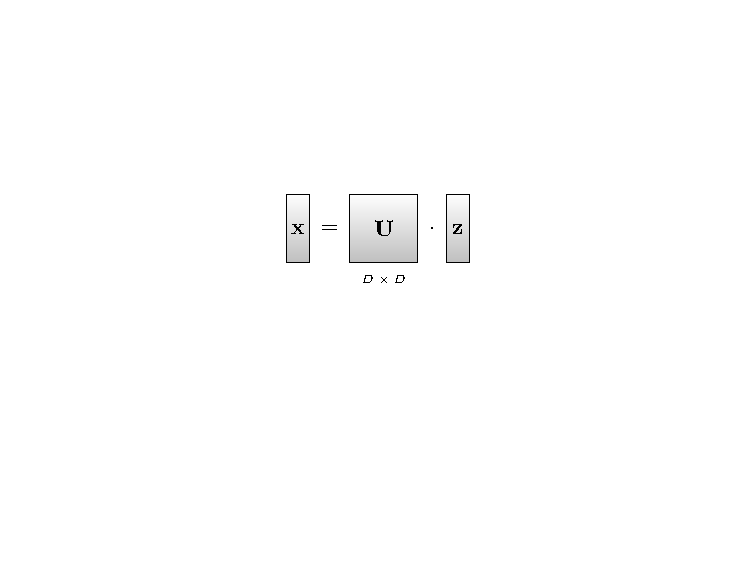
\includegraphics[width=0.5\textwidth,page=1]{img/10_bases}
        \end{figure}
        \subitem Advantage: Efficient coding by matrix multiplication $z = U^Tx$.
        \subitem Disadvantage: Only sparse for a single class of signals.

    \item[Fixed Overcomplete Basis] $\ $
        \begin{figure}[H]
            \centering
            \includegraphics[width=0.5\textwidth,page=2]{img/10_bases}
        \end{figure}
        \subitem Advantage: Sparse coding for several signal classes.
        \subitem Disadvantage: Finding the sparsest code
            \begin{itemize}
            \item Requires an approximation algorithm,
            \item Is problematic if the dictionary size is $L$ and the coherence $m(U)$ is large.
            \end{itemize}

    \item[Learning the Dictionary] $\ $
        \subitem Advantage: We adapt the dictionary to signal characteristics and thus get the same approximation error achievable with a smaller $L$.
        \subitem Disadvantage: We have to solve a matrix factorisation problem. 
        \begin{figure}[H]
            \centering
            \includegraphics[width=0.7\textwidth,page=3]{img/10_bases}
        \end{figure}
        subject to sparsity constraint on $Z$ and atom norm constraint on $U$.
\end{description}

\subsubsection{Matrix Factorisation}
\begin{align*}
    (U^*, Z^*) \in \argmin_{U,Z} \norm{X-U\cdot Z}_F^2
\end{align*}
We observe that the objective function is \emph{not convex} in both $U$ and $Z$ (local minima). But convex in either $U$ or $Z$ (unique minimum).
\paragraph{Iterative Greedy Minimisation} $\ $
\begin{enumerate}
    \item Initialisation
    
        The minimisation is sensitive to the choice of $U^0$: The initial candidate solution is optimised locally and greedily until no progress is possible.
        \begin{description}
            \item \emph{Random atoms}:
            
                Sample $\{u_l^0\}$ on the unit sphere:
                \begin{enumerate}
                    \item Sample $D$ dimensional standard normal distribution:
                        \begin{align*}
                             u_l^0 \sim \mathcal N (0,ID).
                        \end{align*}
                    \item Scale to unit length:
                        \begin{align*}
                            u_l^0 \gets {u_l^0 \over  \norm{u_l^0}_2}.
                        \end{align*}
                \end{enumerate}
            \item \emph{Samples from $X$}:
                \begin{enumerate}
                    \item $u_l^0\gets x_n$, where $n\sim \mathcal U(1,N)$ is sampled uniformly.
                    \item Scale to unit length:
                        \begin{align*}
                            u_l^0 \gets {u_l^0 \over  \norm{u_l^0}_2}.
                        \end{align*}
                \end{enumerate}
        \end{description}
        Use \emph{fixed overcomplete dictionary}, e.g. overcomplte DCT.
    \item Coding step:
        \begin{align*}
             Z^{t+1} \in \argmin_Z \norm{X-U^t\cdot Z}_F^2,
        \end{align*}
        subject to $Z$ being sparse and fixed $U$.
        
        Since each column is separable we get:
        \begin{align*}
            \norm{R}_F^2 = \sum_{i,j} r_{i,j}^2 = \sum_j \norm{r_j}_2^2.
        \end{align*}
        Thus we obtain $N$ \emph{independent} sparse coding steps:
        \begin{align*}
            z_n^{t+1} &\in \argmin_z \norm{z}_0,
            \text{s.t. }\ &\norm{x_n}
        \end{align*}


    \item Dictionary update step:
        \begin{align*}
            U^{t+1} \in \argmin_U \norm{X-U\cdot Z}_F^2,
        \end{align*}
        subject to $\norm{u_l}_2 - 1\ \forall l\in[1,L]$ and fixed $Z$.
        
        In contrast to the coding step the residual is \emph{not separable} in atoms (columns of $U$).
        
        \emph{Approximation}: Update on atom at a time. $\forall l\in[1,L]$:
        \begin{enumerate}
            \item Set $U = [u_1\ldots u_l\ldots u_L^t]$ fix for all atoms except $u_l$.
            \item Isolate $R_l^t$ that minimises $R_l^t$ subject to $\norm{u_l^*}_2 =1$.
                \begin{align*}
                    &\norm{X-[u_1^t\ldots u_l \ldots u_L^t]\cdot Z^{t+1}}_F^2\\
                    =&\norm{
                        X-\left(
                                \sum_{e\neq l} u_e^t (z_e^{t+1})^T + u_l (z_l^{t+1})^T
                            \right) 
                    }_F^2\\
                    =& \norm{R_l^t - u_l (z_l^{t+1})^T}_F^2,
                \end{align*}
                where $z_l^T$ is the $l$-th row of matrix $Z$.
            \item Find $u_l^*$ that minimises $R_l^t$, subject to $\norm{u_l^*}_2 = 1$.
                
                We observe that $u_l(z_l^{t+1})^T$ is an outer product, i.e. a matrix.
                Hence we need to minimise the residual
                \begin{align*}
                    \norm{R_l^t - u_l (z_l^{t+1})^T}_F^2
                \end{align*}
                by approximating $R_l^t$ with a rank-1 $u_l (z_l^{t+1})^T$.
                
                This is achieved by SVD of $R_l^t$:
                \begin{align*}
                    R_l^t = \tilde U S\tilde V^T = \sum_i s_i \tilde u_i \tilde v_i^T,
                \end{align*}
                $u_l^* = \tilde u_1$ being the first left-singular vector. 
                
                We also observe that $\norm{u_l^*} =1$ is naturally satisfied.
        \end{enumerate}
\end{enumerate}









































\newpage
\section{Robust Principal Component Analysis}
Goal: Find a low rank representation of a matrix $X$, which is corrupted by a sparse perturbation or sparse structured noise.
\begin{figure}[H]
\centering
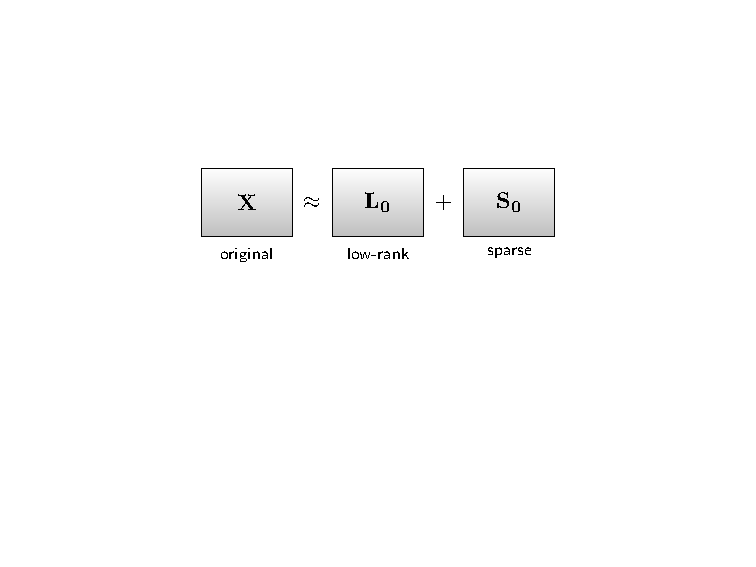
\includegraphics[width=.8\textwidth]{img/11_rpca}
\end{figure}
In contrast to the topic we have discussed so far we have compute a \emph{additive decomposition}.

\subsection{Additive Decomposition Problem}
\begin{align*}
     \text{minimise}\ &rank(L)+\lambda\cdot card(S)\\
     \text{subject to}\ &L+S =X,
\end{align*}
where $card(\cdot)$ counts the number of non-zero entries.

This optimisation problem formalises the notion of separating a matrix into a low-rank and a sparse one. However, this decomposition is difficult to compute in general. For instance, it is not a convex optimisation problem.

\subsection{Principal Component Pursuit (PCP)}
\begin{align*}
     \text{minimise}\ &\norm{L}_* +\lambda \norm{S}_1,
     \text{subject to}\ &L+S =X,
\end{align*}
where $\norm{\cdot}$ denotes the nuclear norm:
\begin{align*}
    \sum_{i=1}^{\min\{m,n\}} \sigma_i,
\end{align*}
where $\sigma_i$ denotes the $i$'th singular value of a $n\times m$ matrix and $\norm{\cdot}_1$ denotes the sum of absolute values of all matrix entries.

Note that this is not the same problem as minimising $rank(L) + \lambda\cdot card(S)$. The $L1$-Norm is only a convex relaxation of cardinality and the nuclear norm a convex relaxation of the rank.


But this relaxation will allow us to efficiently solve the problem, and if we are fortunate (i.e. under some conditions on the sparsity and low-rankness of our matrices) we recover the original matrices. We will see that this coincidence of solutions happens under surprisingly broad conditions.


In contrast to the additive decomposition problem, \emph{PCP} is \emph{convex}.

\subsection{Lagrange Mutlipliers} $\ $
\subsubsection{Primal Optimisation Problem}
\begin{align*}
    \text{minimise}\ &f(x)\\
    \text{subject to}\ &g_i(x)\leq 0&i\in[1,m]\\
     &h_i(x) =0 &i\in[1,p]
\end{align*}
\subsubsection{Unconstrained Problem} $\ $
\begin{align*}
    \text{minimise}\ &f(x) + \sum_{i=1}^m I_- (g_i(x)) + \sum_{i=1}^p I_0(h_i(x))\\
        I_-(u) &= \begin{cases}
                     0 &u\leq 0\\
                     \infty &u>0
                 \end{cases}\\
        I_0(u) &=
            \begin{cases}
                0 & u=0\\
                \infty &u\neq 0
            \end{cases}
\end{align*}
$I_0$ and $I_-$ penalise perturbations with violating constraints by "brick wall" penalty functions.

We can approximate $I_-(u)$ linearly with $\lambda_i u, \lambda_i \geq 0$ and $I_0(u)$ with $\nu_i u$:

\begin{align*}
    I_-(u) &\approx \lambda_i u &\lambda_i \geq 0\\
    I_0(u) &\approx \nu_i u,
\end{align*}
where $\lambda_i$ and $\nu_i$ are called Lagrange multipliers.

\paragraph{Lagrangian} \
\begin{align*}
    L(x,\lambda, \nu) =  f(x) + \sum_{i=1}^m \lambda_i g_i(x) + \sum_{i=1}^p \nu_i h_i(x).
\end{align*}
\paragraph{Lagrange dual function} \
\begin{align*}
    d(\lambda, \nu) = \inf_x L(x,\lambda, \nu).
\end{align*}

Since $\lambda_i u\leq I_-(u)$ and $\nu_i u\leq I_0 (u)$ for all $u$: The dual function is a lower bound on the optimal value of the primal problem $p^*$.
\begin{figure}[H]
    \centering
    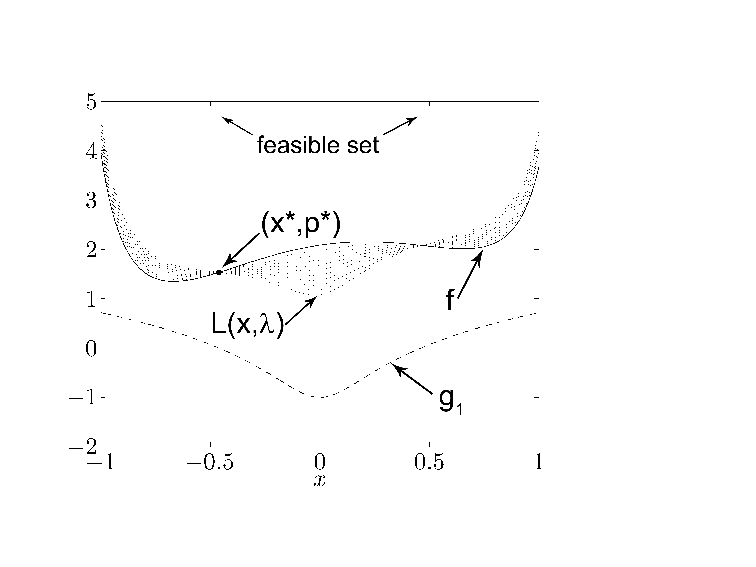
\includegraphics[width=0.7\textwidth]{img/11_lagrangian_dual_function_lower_bound}
\end{figure}

\subsection{Dual Problem}
\begin{description}
    \item[Lagrangian] \
        \begin{align*}
                L(x,\lambda, \nu) =  f(x) + \sum_{i=1}^m \lambda_i g_i(x) + \sum_{i=1}^p \nu_i h_i(x).
        \end{align*}
    \item[Lagrangian Dual Function] \
        \begin{align*}
            d(\lambda, \nu) = \inf_x L(x,\lambda, \nu).
        \end{align*}
        Now find the best lower bound on $p^*$:
    \item[Lagrange dual problem] \ 
        \begin{align*}
            \text{maximise}\ &d(\lambda, \nu)\\
            \text{subject to}\ &\lambda \geq 0
        \end{align*}
\end{description}

\emph{Strong Duality} If the primal optimisation problem is convex, under some conditions, the solution to the dual problem is equivalent to the solution of the primal problem.
It is always a lower bound on the solution of the primal problem.

In order to compute the additive decomposition for RPCA we will introduce a method called \emph{Alternating Direction Method of Multipliers}. This method builds upon two other methods, whose positive features it combines: Dual decomposition and method of multipliers.
\subsection{Convex Optimisation with Equality Constraints}
\begin{align*}
    \text{minimise}\ &f(x)\\
    \text{subject to}\ &Ax=b.
\end{align*}
\begin{description}
\item Lagrangian: $L(x,\nu) = f(x) + \nu^T (Ax-b)$
\item Dual function: $d(\nu) =\inf_x L(x,\nu)$
\item Dual problem: $\text{maximise}\ d(\nu)$
\item Recover optimal $x:\ x^*\in\argmin_x L(x,\nu^*)$ 
\end{description}

\paragraph{Gradient Method for Dual Problem}\
\begin{align*}
    \nu^{k+1} &= \nu^k +\alpha^k\nabla d(\nu^k)\\
    \nabla d(\nu^k) &= A\tilde x-b\\
    \tilde x &= \argmin_x L(x,\nu^k),
\end{align*}
\begin{itemize}
    \item $\nabla d$: Gradient of the dual function.
    \item $\alpha^k$: Step length at step $k$.
\end{itemize}

\paragraph{Dual Decomposition}
Goal: Parallelise individual optimisation steps on a cluster. 
\begin{description}
\item Suppose $f(x)$ is separable
    \begin{align*}
         f(x) &= f_1(x_1) + \ldots + f_N(x_N) &x=(x_1,\ldots, x_N)
    \end{align*}
\item Now $L$ is separable
    \begin{align*}
        L(x,\nu) &= L_1(x_1,\nu) + \ldots + L_N (x_n,\nu) - \nu^T b\\
        L_i(x_i,\nu) &= f_i(x_i) + \nu^T A_ix_i.
    \end{align*}
\item Split $x$-minimisation step and we get the dual decomposition:
    \begin{align*}
        x_i^{k+1} &:= \argmin_{x_i} L_i (x_i,\nu^k) &i\in[1,N]\\
        \nu^{k+1} &:= \nu^k + \alpha^k 
            \left(
                A_i x_i^{k+1} -b
            \right)
    \end{align*}
\item Parallelisable Algorithm:
    \begin{algorithmic}
        \STATE init $\nu^1$ and $x^1$
        \FOR{$k=2,\ldots,K$}
            \FOR{$i=1,\ldots,N$}
                \STATE // this can be parallelised
                \STATE $x_i^{k+1} :=\argmin_{x_i} L_i(x_i,\nu^k)$ $i=1,\ldots N$
                \STATE $\Theta^{k+1} = A_i x_i$
            \ENDFOR
            \STATE $\nu^{k+1} := \nu^k +\alpha^k \left(\sum_{i=i}^N \Theta^{k+1} -b\right)$ \todo{$i$ missing in $\Theta$?}
        \ENDFOR
        \STATE return $x^{k+1}$
    \end{algorithmic}
    
\end{description}

\subsection{Method of Multipliers}
To overcome some problems of Dual ascent, namely convergence only under strict convexity and finiteness of $f$ we introduce:
\paragraph{Augmented Lagrangian} \
\begin{align*}
    L_\rho (x,\nu) = f(x) + \nu^T (Ax-b)+ {\rho\over 2} \norm{Ax-b}_2^2,
\end{align*}
for any feasible $x:\ L_\rho (x,\nu) = L(x,\nu)$.
\paragraph{Method of Multipliers} \
\begin{align*}
    x^{k+1} &:= \argmin_x L_\rho(x,\nu^k)\\
    \nu^{k+1} &= \nu^k+\rho (Ax^{k+1} -b)
\end{align*}
This adds more penalty to for violating the constraints and converges under far more general conditions than dual ascent.
\subsubsection{Dual Update Step $\mathbf \rho$} Why choose $\rho$ as step size?
\paragraph{Optimality Conditions} Primal and dual feasibility
\begin{align*}
    Ax^* - b &= 0\\
    \nabla f(x^*) +A^T\nu^* &= 0.
\end{align*}
By definition $x^{k+1}$ minimises $L_\rho(x,\nu^k)$, so
\begin{align*}
    0 &= \nabla_x L_\rho (x^{k+1},\nu^k)\\
    &= \nabla_x f(x^{k+1}) +  A^T (\nu^k+\rho(Ax^{k+1} -b))\\
    &= \nabla_x f(x^{k+1}) + A^T \nu^{k+1}
\end{align*}

Therefore using $\rho$ as step size the iterate $(x^{k+1}, \nu^{k+1})$ is dual feasible. The primal residual $Ax^{k+1} -b$ converges to zero as the method of multipliers proceeds.

\subsection{Alternating Directions Method of Multipliers (ADMM)}
The main disadvantage of the method of multipliers is that the augmented Laplacian is not separable anymore. Hence we can not parallelise the $x$-minimisation step.

To get the superior convergence properties of the method of multipliers and the decomposability of dual ascent, we finally introduce the \emph{Alternating Direction Method of Multipliers} (ADMM). The method splits the variable $x$ into two parts, with the objective function separable over this splitting. The algorithm then separately minimises the two primal variables $x$ and $z$.
\begin{align*}
    \text{minimise }&f(x)+p(x) & f,\ p\text{ convex}\\
    \text{subject to }&Ax+Bz = c.
\end{align*}
\paragraph{Augmented Lagrangian} \
\begin{align*}
    L_\rho(x,z,\nu) = f(x) + p(z) +\nu^T (Ax+Bz-c) + {\rho\over 2}\norm{Ax+Bz-c}_2^2.
\end{align*}
\paragraph{ADMM}\
\begin{align*}
    x^{k+1} &:= \argmin_x L_\rho (x, z^k, \nu^k)\\
    z^{k+1} &:= \argmin_z L_\rho (x^{k+1}, z, \nu^k)\\
    \nu^{k+1} &:= \nu^k +\rho(Ax^{k+1}+Bz^{k+1}-c)
\end{align*}

\subsubsection{Optimality Conditions}
\begin{description}
\item \emph{Primal Feasibility}
    \begin{align*}
        Ax^* + Bz^* -c = 0.
    \end{align*}
\item \emph{Dual Feasibility}
    \begin{align*}
        \nabla f(x^*) +A^T \nu^* &= 0\\
        \nabla p(z^*) +B^T \nu^* &= 0
    \end{align*}
\end{description}
These primal and dual feasibility conditions are the \emph{necessary} and \emph{sufficient} optimality conditions for the ADMM problem.
It can be shown that the residual of the other two feasibility conditions converge to zero as ADMM proceeds.\\


We will show that $z^{k+1}$, one of the two primal variables, and $\nu^{k+1}$, the dual variable always satisfy the second dual feasibility condition.

\begin{align*}
    \nabla_z L_\rho (x,z,\nu) = \nabla_z p(z) + B^T \nu +\rho B^T(Ax+Bz-c)
\end{align*}
Since $z^{k+1}$ minimises $L_\rho (x^{k+1},z,\nu^k)$ by definition we have that
\begin{align*}
     0 &= \nabla_z p(z^{k+1}) + B^T \nu^k +\rho B^T (Ax^{k+1}+Bz^{k+1}-c)\\ 
     &= \nabla_z p(z^{k+1}) + B^T(\nu^k+\rho (Ax^{k+1}+Bz^{k+1}-c))\\
     &= \nabla_z p(z^{k+1}) + B^T \nu^{k+1}
\end{align*}
We observe that $z^{k+1}$ and $\nu^{k+1}$ always satisfy:
\begin{align*}
        \nabla p(z^*) +B^T \nu^* &= 0
\end{align*}

\subsection{Robustness}
\subsubsection{Classical PCA}
Classical PCA is very sensitive to outliers. \emph{One single} grossly corrupted point completely changes the principal components.
\begin{figure}[H]
    \centering
    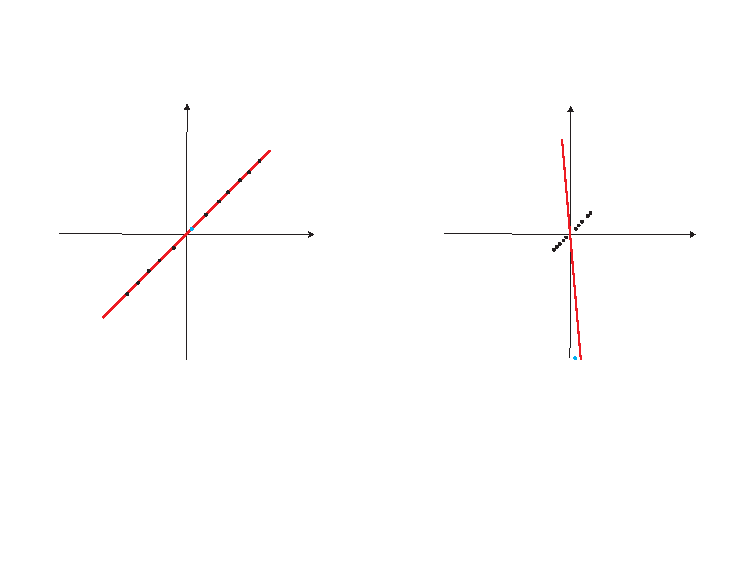
\includegraphics[width=0.7\textwidth]{img/12_pca_robustness}
\end{figure}

The main reason is that the sum of squares is minimised:
\begin{align*}
    {1\over N} \sum_{n=1}^N \norm{x_n-\tilde x_n}_2^2.
\end{align*}

\subsection{Robust PCA}
RPCA explicitly models the errors as sparse noise due to separation into low-rank and sparse matrices:
\begin{align*}
\text{minimise}\ &rank(L) + \lambda \cdot card(S)\\
\text{subject to}\ &L+S=X
\end{align*}
which can be modelled by the principal component pursuit.
\begin{align*}
    \text{minimise}\ &\norm{L}_* + \lambda \norm{S}_1\\
    \text{subject to}\ &L+S=X,
\end{align*}
where $\norm{\cdot}_*$ denotes the nuclear norm and $\norm{\cdot}$ denotes the $L_1$-norm of $S$ seen as a vector.

\paragraph{Advantages} RPCA is robust to grossly corrupted observations of $X$. It does not need to know the sparsity pattern of $S_0$. Can be easily extended to matrix completion.

\paragraph{Applications where large errors frequently occur} are
\begin{description}
    \item \emph{Image processing}: Salt \& Pepper noise
    \item \emph{Web data analysis}: Adversarial information
    \item \emph{Bioinformatics}: Spurious errors in measurements and sensor failures.
    \item \emph{Computer Vision}: Occlusions
\end{description}

\subsubsection{Recovery of $L_0$ and $S_0$}
Find the decomposition of $X$ into low rank and sparse matrix $X=L_0+S_0$:


Principal Component Pursuit (PCP):
\begin{align*}
    \text{minimise}\ &\norm{L}_* + \lambda \norm{S}_1\\
    \text{subject to}\ &L+S=X,
\end{align*}
Under broad conditions the recovery is perfect, i.e. the solution $(L^*, S^*)$ obeys:
\begin{align*}
    L^*  &= L_0,
    S^*  &= S_0.
\end{align*}

\begin{itemize}
    \item $X$ can not be low-rank and sparse.
    \item $L_0$ can not be sparse:
        \begin{align*}
            L_0 \in \R^{n\times n} &= U\Sigma M^T = \sum_{1\leq i\leq r} \sigma_i u_i v_i^T &r = rank(L_0)\\
            e_i &= (0,\ldots,0,1,0,\ldots,0)
        \end{align*}
    \item Coherence condition:
        \begin{align*}
            \norm{U^T e_i}^2 &\leq {\mu r\over n}\\
            \norm{M^T e_i}^2 &\leq {\mu r\over n}\\
            |UM^T|_{ij}^2 &\leq {\mu r\over n^2}
        \end{align*}
        This means, that Principal Components can not be sparse (spiky).
\end{itemize}

\subsubsection{Theorem}
For 
\begin{description}
\item $L_0$: $n \times n$, of $rank(L_0) \leq \rho_r n\mu^{-1}(\log n)^{-2}$
\item $S_0$: $n \times n$, random sparsity pattern of cardinality $n\leq \rho_s n^2$.

    $\rho_s$, $\rho_r$ are positive constraints.
\end{description}
With probability $1-\bigO{n^{-10}}$, PCP with $\lambda = {1\over \sqrt{n}}$ is exact.
The same holds for rectangular matrices with $\lambda= {1\over \sqrt{\max(n,m)}}$.

\subsection{Solving Robust PCA}
We want to solve
\begin{align*}
    \text{minimise}\ &\norm{L}_* + \lambda \norm{S}_1\\
    \text{subject to}\ &L+S=X.
\end{align*}
This can now be easily solved using ADMM:

We have chosen $f(x) = \norm{L}_*$ and $p(z) = \norm{S}_1$:
\begin{align*}
    L_\mu (L,S,N) &= \norm{L}_* +\lambda \norm{S}_1 + \langle N, (X-L-S)\rangle +{\mu\over 2} \norm{X-L-S}_F^2\\
    \text{with }\langle X,Y\rangle &\text{ being the Frobenius inner product: }\sum_i\sum_j X_{ij}Y_{ij}.
\end{align*}

\paragraph{ADMM for RPCA:} \
\begin{align*}
    L^{k+1} &:= \argmin_L L_\mu(S,L^k,N^k)\\
    S^{k+1} &:= \argmin_S L_\mu(S^{k+1}, L,N^k)\\
    N^{k+1} &:= N^k +\mu(X-L^{k+1}-S^{k+1})
\end{align*}
We observe that we can solve the minimisation over $L$ and $S$ explicitly:
\begin{align*}
    \argmin_S L_\mu (S,L,N) &=\mathcal S_{\lambda \mu^{-1}} (X-L+\mu^{-1}N)\\
    \argmin_L L_\mu (S,L,N) &=\mathcal D_{\mu^{-1}}(X-S+\mu^{-1}N)
\end{align*}
with
\begin{align*}
    \mathcal S_\tau(x) &= \text{sgn}(x)\max(|x|-\tau,0)\\
    \mathcal S_\tau(X) &: \text{Apply $\mathcal S_\tau$ to each element}\\
    \mathcal D_\tau(X) &= U\mathcal S_\tau (\Sigma) M^T\\
    text{where SVD } X &= U\Sigma M^T
\end{align*}

Combining all of the above we get an algorithm to solve robust PCA:


\begin{algorithmic}
    \STATE $S_0:= 0$
    \STATE $\nu_0 :0$
    \STATE $\mu > 0$
    \WHILE{not converged}
        \STATE $L^{k+1} := \mathcal D_{\mu^{-1}} (X-S^k + \mu^{-1} N^k)$
        \STATE $S^{k+1} := \mathcal S_{\lambda \mu^{-1}} (X-L^{k+1} +\mu^{-1} N^k)$
        \STATE $N^{k+1} := N^k +\mu(X-L^{k+1}-S^{k+1})$
    \ENDWHILE
\end{algorithmic}










 


























\newpage
\appendix
 
\part{Appendix}
\section{Matrix Definitions and Theorems}
\subsection{Norms}
A \emph{norm} is a function $\norm{\circ}: V \mapsto \R$ quantifying the size of a vector. It must satisfy
\begin{itemize}
    \item \emph{Positive scalability:}
    \begin{align*}
        \norm{a\cdot x} &= |a|\cdot \norm{x}.
    \end{align*}
    \item \emph{Triangle inequality}
    \begin{align*}
        \norm{x+y} \leq \norm{x} + \norm{y} \quad \forall x,y \in V.
    \end{align*}
    \item \emph{Separability}:
    \begin{align*}
        \norm{x} = 0 \ \implies \ x=0.
    \end{align*}
\end{itemize}
\subsubsection{Vector norms}
\begin{description}
    \item[$\mathbf{p}$-norms] The most commonly used matrix norms are $p$-norms.
        \begin{align*}
            \norm{x}_p := \left(\sum_{i-1}^n |x_i|^p\right)^{1/p}
        \end{align*}
        for $p \in [1,\infty]$, where $|x_i|$ denotes the absolute value of coordinate $x_i$.
        
        A special case of the $p$ norm is the \emph{Eclidean norm}:
        \begin{align*}
            \norm{x}_2:= \sqrt{\sum_{i=1}^n x_i^2}.
        \end{align*}
    \item[$0$-norm] technically not really a norm is defined by:
        \begin{align*}
            \norm{x}_0 := \text{number of nonzero coordinates in $x$}.
        \end{align*}
\end{description}
\subsubsection{Matrix norms}
\begin{description}
    \item[$p$-norm] for matrices:
        \begin{align*}
            \norm{X}_p := \max_{x\neq 0} {\norm{Ax}_p \over \norm{x}_p}.
        \end{align*}
        A special case is the Euclidean or \emph{spectral norm}:
        \begin{align*}
            \norm{X}_2 = \sigma_\text{max} (X),
        \end{align*}
        the largest singular value of $X$.
    \item[Frobenius norm] is defined as:
        \begin{align*}
            \norm{X}_F := \sqrt{\sum_{i=1}^m \sum_{j=1}^n x_{ij}^2} = \sum_{i=1}^{\text{min}(m,n)} \sigma_i^2,
        \end{align*}
        where $\sigma_i$ are the singular values of $X$.
        
        
\end{description}

\subsection{Orthogonality}
\begin{description}
    \item[Orthogonal vectors] Two vectors in an inner product are orthogonal if their inner product is zero.
    \item[Orthonormal vectors] Orthogonal vectors that have unit length 1
    \item[Orthogonal matrix] An orthogonal matrix is a square matrix with real entries whose columns and rows are orthogonal unit vectors (i.e. orthonormal vectors).
    For orthogonal matrices it also holds that
    \begin{align*}
        A^T A= I \quad \implies \quad A^T = A^{-1}\ &\text{since,}\\
        (A^TA)_{i,j} &= a_i^Ta_j = 
            \begin{cases}
                1&i=j\\
                0&i\neq j
            \end{cases}
    \end{align*}

\end{description}


\end{document}
